\documentclass{article}
\usepackage{amsmath}
\usepackage{amsfonts}
\usepackage{graphicx}
\usepackage{url}
\usepackage{float}

\author{Lucija Fekonja}
\title{Projektna naloga iz statistike}

\newcommand{\R}{\mathbb{R}}
\newcommand{\N}{\mathbb N}
\newcommand{\Z}{\mathbb Z}
\newcommand{\C}{\mathbb C}
\newcommand{\Q}{\mathbb Q}



% Še neke ostale stvari ...


\begin{document}

\maketitle

\section*{1. naloga: Kibergrad}
Na podlagi enostavnega vzorca $400$ enot želimo oceniti povprečen dohodek.
Vzorec je enostaven, če iz populacije $N$ enot, v našem primeru je $N = 43886$,
izberemo vzorec, ki ga sestavljajo enote $K_1 \dots K_n \in \left\{ 1 \dots N \right\}$,
kjer je $n = 400$, pri čemer so vsi možni vzorci enako verjetni. V datoteki 
\path{Kibergrad.xlsx} sem enostavni slučani vzorec tvorila tako, da sem vsaki vrstici 
predpisala naključno število med $1$ in $110 \approx N / n$. Nato sem filtrirala 
po tem stolpcu in izbrala tisto skupino med 1 in 110, v katero spada natanko 400 vrstic. 
Če taka skupina ni obstaja, sem postopek ponovila.

Zanimajo nas vrednosti v stolpcu DOHODEK. Na celotni populaciji jih označimo
z $x_1 \dots x_N$, vrednosti na vzorcu pa z $X_1 \dots  X_n$. Tukaj je 
$X_i = x_{K_i}\text{, } i = 1 \dots n$. Ocena za pričakovan dohodek se v teh oznakah
poračuna kot:
$$ \hat{\mu} = \overline{X} = \frac{X_1 + \cdots + X_n}{n} \approx 41047{,}565 \text{.}$$

Da ocenimo standardno napako naše ocene, moramo oceniti še standardni odklon. Na predavanjih 
smo izpeljali, da je 
$$ \hat{\sigma} = \sqrt{\frac{N-1}{N} \frac{1}{n-1} \sum_{i=1}^{n} \left( X_i - \bar{X} \right)^2} \approx 31604{,}637$$
nepristranska cenilka zanjo kadar iz populacije vzamemo enostavni slučajni vzorec. Nato izračunamo oceno standardne napake
$$ \widehat{\text{SE}} = \sqrt{\frac{N-n}{N-1}} \frac{\hat{\sigma}}{\sqrt{n}} = 1573{,}032\text{.}$$

Zadnji del (a) naloge nas sprašuje po konstrukciji intervala zaupanja. Ker $\sigma$
ni znan, ga moramo oceniti, kot smo to storili zgoraj. Za velike $n$ je slučajna
spremenljivka $\frac{\overline{X} - \mu}{\hat{\sigma}} \sqrt{n}$ porazdeljena približno standardno normalno.
%spremenljivka $\left( n - 1 \right) \frac{\hat{\sigma}^2}{\sigma^2} = \frac{1}{\sigma^2}
%\sum_{i=1}^{n} \left( X_i - \overline{X} \right)^2$ pa s porazdelitvijo $\chi^2 \left( n - 1 \right)$.
%Omenjeni slučajni spremenljivki sta neodvisni, zato vemo, da je njun kvocient 
%porazdeljen s Studentovo porazdelitvijo. 
Označimo jo z
$$ Z := \frac{\overline{X} - \mu}{\hat{\sigma}} \sqrt{n} \sim \Phi\left( 0, 1\right) \text{.}$$
Sedaj moramo najti tisti $\delta$, za katerega bo veljalo 
$\overline{X} - \delta \leq \mu \leq \overline{X} + \delta$ v $95\%$ primerov.
Pri stopnji tveganja $\alpha$ je to najmanjši $\delta$, za katerega je 
\begin{align*}
    P \left( | \overline{X} - \mu | \geq \delta \right) &\leq \alpha \\
    P \left( |Z| \geq \frac{\delta}{\hat{\sigma}} \sqrt{n} \right) &\leq \alpha \\
    2 P \left( Z \geq \frac{\delta}{\hat{\sigma}} \sqrt{n}  \right) &\leq \alpha \\
    2 \left( 1 - \Phi \left( \frac{\delta}{\hat{\sigma}} \sqrt{n}  \right)\right) &\leq \alpha \\
    \frac{\hat{\sigma}}{\sqrt{n}} \Phi^{-1} \left( 1 - \frac{\alpha}{2} \right) &\leq \delta \text{.}
\end{align*}
To pomeni, da je iskani interval zaupanja 
$$ \overline{X} - \frac{\hat{\sigma}}{\sqrt{n}} \Phi^{-1} \left( 1 - \frac{\alpha}{2} \right) \leq 
\mu \leq \overline{X} + \frac{\hat{\sigma}}{\sqrt{n}} \Phi^{-1} \left( 1 - \frac{\alpha}{2} \right)$$
oziroma
$$ \mu \in \left[ 37964{,}423, 44130{,}707 \right] \text{.}$$

V (b) delu naloge stratificiramo po četrteh. To pomeni, da populacijo 
razdelimo na stratume, v našem primeru je stratum določena četrt, iz katerih neodvisno izberemo 
enostavni vzorec. Pri izboru enostavnega vzorca iz vsakega od stratumov sem uporabila isto metodo 
kot v (a) delu naloge. Naj $N_l$, $l = 1 \dots 4$ označuje velikost $l$-tega stratuma, $n_l$ pa velikost 
vzorca vzetega iz $l$-tega stratuma. Velikosti $n_l$ določimo s proporcionalno alokacijo,
pri kateri je $n_l = n \frac{N_l}{N} = n W_l$. Tukaj z $W_l$ označujem delež populacije v 
$l$-tem stratumu. V našem primeru poračunamo:

\begin{equation*}
    \begin{aligned}[c]
        n_1 &= n \frac{10149}{N} \approx 92 \text{,}\\
        n_2 &= n \frac{10390}{N} \approx 95\text{,}
    \end{aligned}
    \qquad
    \begin{aligned}
        n_3 &= n \frac{13457}{N} \approx 123 \text{,}\\
        n_4 &= n \frac{9890}{N} \approx 90\text{.}
    \end{aligned}
\end{equation*}
Pričakovana vrednost dohodka $l$-tega stratuma je določena z 
$$ \overline{X}_l = \frac{1}{n_l} \sum_{i=1}^{n_l} X_{il} \text{,}$$
kjer $X_{il}$ označuje $i$-to vrednost v $l$-tem stratumu. V našem primeru je
\begin{equation*}
    \begin{aligned}[c]
        \overline{X}_1 = 44710{,}065\text{,}\\
        \overline{X}_2 = 41644{,}432\text{,}
    \end{aligned}
    \qquad
    \begin{aligned}
        \overline{X}_3 = 34026{,}423 \text{,}\\
        \overline{X}_4 = 37798{,}444\text{.}
    \end{aligned}
\end{equation*}
Ocena pričakovanega dohodka populacije je
$$ \overline{X} = \sum_{l=1}^{4} \frac{N_l}{N} \overline{X}_l = \sum_{l=1}^{4} W_l \overline{X}_l = 39150{,}715 \text{.}$$
Da dobljen rezultat primerjamo z enostavnim slučajnim vzorčenjem, je potrebno pogledati 
standardno napako ocene. Zanjo pa potrebujemo varianco vsakega od stratumov, ki jo 
izračunamo na naslednji način:
$$ \hat{\sigma}_l^2 = \frac{N_l - 1}{N_l} \frac{1}{n_l - 1} \sum_{i=1}^{n_l} \left( X_{il} - \overline{X}_l \right)^2 \text{.}$$
Po danih podatkih je
\begin{equation*}
    \begin{aligned}[c]
        \hat{\sigma}_1 = 32635{,}808\text{,}\\
        \hat{\sigma}_2 = 39578{,}556\text{,}
    \end{aligned}
    \qquad
    \begin{aligned}
        \hat{\sigma}_3 = 26916{,}903 \text{,}\\
        \hat{\sigma}_4 = 22674{,}367\text{.}
    \end{aligned}
\end{equation*}
Varianca povprečnega dohodka populacije stratificirane s proporcionalno alokacijo 
je izračunana kot
$$ Var \left( \overline{X} \right) = \sum_{l=1}^{4} \frac{W^2_l \hat{\sigma}_l^2}{n_l} \text{.}$$
Potem je standarna napaka ocene povprečja enaka
$$ \widehat{SE} = \sqrt{Var \left( \overline{X} \right)} = 1545{,}099
 \text{.}$$
Standardna napaka je pri stratificiranem vzorčenju manjša kot pri enostanvem slučajnem 
vzorčenju, kar pomeni, da smo v (b) primeru dobili nekoliko boljšo oceno za pričakovan 
dohodek. Stratificirano vzorčenje da boljšo oceno za pričakovano vrednost, če se
vrednosti znotraj posameznih stratumov ne razlikujejo veliko, medtem ko so med različnimi
stratumi razlike velike. V dani populaciji Kibergrada se dohodki znotraj stratumov precej 
razlikujejo, prav tako pa med različnimi stratumi težko ločimo. Zato ocena s stratificiranim
vzorčenjem ni veliko boljša od ocene pri enostavnem vzorčenju.


\section*{2. naloga: Kevlar}
Primerjalni kvantilni (Q--Q) grafikon je v splošnem sestavljen iz točk $(x, y)$, kjer $x$
teče po vseh kvantilih prve, $y$ pa po vseh kvantilih druge porazdelitve za vsako verjetnost 
$\alpha \in \left( 0, 1\right)$. Ko primerjamo teoretično in empirično porazdelitev prikažemo
le kvantile za verjetnosti $\frac{1}{n + 1} \dots \frac{n}{n + 1}$, kjer je $n$ število opaženih
podatkov. Opažanja uredimo v ražirno vrsto $X_{\frac{1}{n+1}} \leq \dots \leq X_{\frac{n}{n+1}}$, 
kar je v \url{Kevlar.xlsx} že dano. 

Naloga od nas zahteva, da empirično porazdelitev primerjamo z eksponentno. Za prikaz primerjalnega
kvantilnega grafikona bomo potrebovali kumulativno funkcijo eksponentne porazdelitve, to je 
$$ F(x) =
\begin{cases}
    1 - e^{- \lambda x}, & x \geq 0, \\
    0, & x < 0 \text{.}
\end{cases}
$$
Vzemimo $\lambda = 1$.
Naj bodo $X_1 \dots X_n, n = 101,$ dana opažanja trajanja vlaken pri $90\%$ obremenitvi, preden je prišlo 
do porušitve. Za vsak $k = 1 \dots n$ narišemo točke
$$ \left( \frac{k}{n + 1}, F \left( X_k \right)\right) \text{.}$$

\begin{figure}[H]
    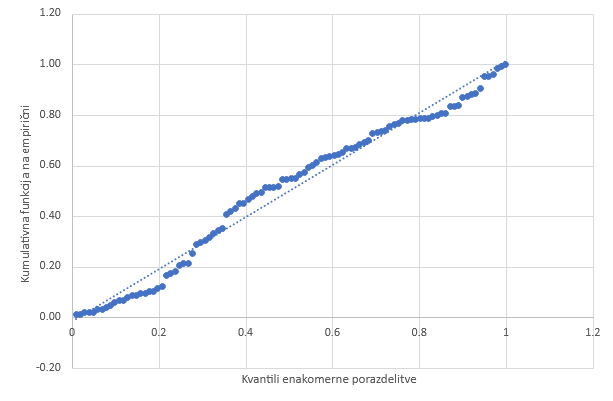
\includegraphics[height=8cm]{qq-1.png}
    \caption{Primerjalni kvantilni (Q--Q) grafikon, ki enakomerno porazdeljenim $n$ točkam na intervalu $(0, 1)$ priredi vrednosti kumulativne funkcije eksponentne porazdelitve.}
\end{figure}
Vidimo, da se empirični podatki ujemajo z eksponentno porazdelitvijo, saj je dobljen graf
skoraj linearen. Črta, ki se podatkom najbolje prilega ima enačbo $y = 1{,}0228 x - 0{,}0197$.
Oglejmo si še ekvivalentno konstrukcijo primerjalnega kvantilnega grafikona, 
v kateri za vsak $k = 1 \dots n$ narišemo točke
$$ \left( F^{-1} \left( \frac{k}{n+1}\right), X_k \right) \text{.}$$
\begin{figure}[H]
    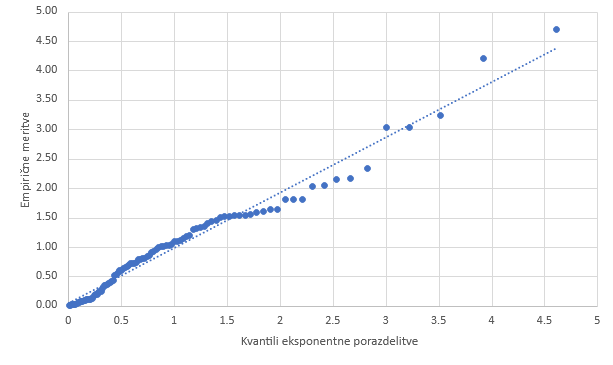
\includegraphics[height=8cm]{qq-2.png}
    \caption{Primerjalni kvantilni (Q--Q) grafikon predstavljen s točkami $ \left( F^{-1} \left( \frac{k}{n+1}\right), X_k \right)$.}
\end{figure}
Tudi v tem primeru se empirična porazdelitev ujema z eksponentno, saj je črta, ki se podatkom najbolje 
prilega linearna. Njena enačba je $y = 0{,}9401 x - 0{,}0361$. Sklepamo, da je trajanje vlaken, 
preden je prišlo do porušitve, porazdeljeno eksponentno.
Namreč ko primerjamo dve eksponentni porazdelitvi, je primerjalni kvantilni grafikon linearen. V bistvu 
je Q--Q grafikon linearen, če primerjamo dve enaki porazdelitvi. 

V nadaljevanju nas naloga sprašuje po eksponentni porazdelitvi, ki se najbolj prilega danim podatkom.
Poiskati moramo torej $\lambda$ v gostoti eksponentne porazdelitve 
$$ f (x | \lambda) = \lambda e^{- \lambda x} $$
po metodi največjega verjetja. Predpostavimo, da so opažanja $x_1 \dots x_n$ neodvisna.
Potem je verjetje definirano kot:
$$ L (\lambda | x) = \prod_{i=1}^{n} f (x_i | \lambda) = \prod_{i=1}^{n} \lambda e^{- \lambda x_i} = \lambda^n e^{- \lambda \sum_{i=1}^{n}x_i} \text{.}$$
Če verjetje logaritmiramo, dobimo 
$$ l (\lambda | x) = n \ln (\lambda) - \lambda \sum_{i=1}^{n}x_i \text{.} $$
Iščemo maksimum verjetja $L$ oz. $l$, zato odvajamo $l$ po $\lambda$, kar nam da 
$\frac{dl}{d\lambda} ( \lambda | x) = \frac{n}{\lambda} - \sum_{i=1}^{n}x_i$, iz česar
izrazimo 
$$ \lambda = \frac{n}{\sum_{i=1}^{n}x_i} = 0{,}976695 \text{.}$$
Porazdelitev, ki se danim podatkom najbolje prilega je torej \emph{Exp($0{,}976695$)}.

Da ugotovimo, če se empirična porazdelitev res prilega eksponentni, lahko narišemo tudi 
viseči histogram iz razlik korenov frekvenc. Pri risanju histograma podatke razdelimo v
razrede, katerih širino lahko izračunamo po npr. modificiranem Freedman--Diaconisovem pravilu, 
pri katerem je $$ \text{širina} = \frac{2.6 \cdot \text{IQR}}{\sqrt[3]{n}}\text{.}$$ V našem primeru je
interkvartilni razmik enak $\text{IQR} = x_{3/4} - x_{1/4} = 1{,}455 - 0{,}235 = 1{,}22$, kjer sta
$x_{1/4}$ in $x_{3/4}$ prvi oz. tretji kvartil.
Širina intervala po zgoraj navedenem pravilu je torej $0{,}242789074$. Naj bo sedaj $x_{j-1}$ 
leva meja $j$-tega intervala, $x_{j}$ pa desna. Verjetnost, da opažanje pade na $j$-ti interval
je 
$$ \hat{p_j} = \int_{\frac{x_{j-1} - \hat{\mu}}{\hat{\sigma}}}^{\frac{x_{j} - \hat{\mu}}{\hat{\sigma}}} \lambda e^{- \lambda x} dx \text{,}$$
kjer sta cenilki $\hat{\mu}$ in $\hat{\sigma}$ izračunani z
$$ \hat{\mu} = \frac{1}{n} \sum_{i=1}^{n} x_i \qquad \text{in} \qquad \hat{\sigma} = \frac{1}{n-1} \sum_{i=1}^{n} \left( x_i - \overline{x} \right)^2 \text{.} $$
Pričakovano število opažanj na $j$-tem intervalu je $\hat{n}_j = n \hat{p_j}$. Označimo z 
$n_j$ dejansko število opažanj na $j$-tem intervalu. Pri visečem histogramu nas zanima razlika
$n_j - \hat{n_j}$, pri visečem histogramu iz razlik korenov frekvenc pa $\sqrt{n_j} - \sqrt{\hat{n_j}}$.
Narišimo oba viseča histograma in podajmo tabeli razlik frekvenc oziroma razlik njihovih korenov.
%\begin{table}[H]
%    \centering
%    \begin{tabular}{c c}
%        \bf{Sredina intervala}  &	$n_j - \hat{n_j}$   \\
%        0.340561899  &	-3.927760008   \\
%        1.021685696  &	4.358188116   \\
%        1.702809493  &	5.33053886   \\
%        2.383933291  &	-2.513938436   \\
%        3.065057088  &	-0.349108023   \\
%        3.746180885  &	-1.721926705   \\
%        4.427304682  &	1.11468022   \\
%        5.10842848   &	-0.455182622   \\
%        5.789552277  &	-0.23402981   \\
%        6.470676074  &	-0.120325226   \\
%        7.151799872  &	-0.061864597   \\
%        7.832923669  &	0.968192635   \\
%        8.514047466  &	-0.016353594   \\
%    \end{tabular}
%    \caption{Tabela vrednosti $n_j - \hat{n_j}$.}
%\end{table}
\begin{table}[H]
    \centering
    \begin{tabular}{c c}
        \bf{Sredina intervala}  &	$n_j - \hat{n_j}$   \\
        0.3406   &  	-151.6958539   \\
        1.0217   &  	-78.90811836   \\
        1.7028   &  	-41.50131883   \\
        2.3839   &  	-28.80945688   \\
        3.0651   &  	-15.09137051   \\
        3.7462   &  	-9.975711295   \\
        4.4273   &  	-3.500678381   \\
        5.1084   &  	-3.033113146   \\
        5.7896   &  	-1.672480053   \\
        6.4707   &  	-0.922217289   \\
        7.1518   &  	-0.508517086   \\
        7.8329   &  	 0.719600124   \\
        8.514    &  	-0.154614444   \\
    \end{tabular}
    \caption{Tabela vrednosti $n_j - \hat{n_j}$.}
\end{table}
\begin{figure}[H]
    \centering
    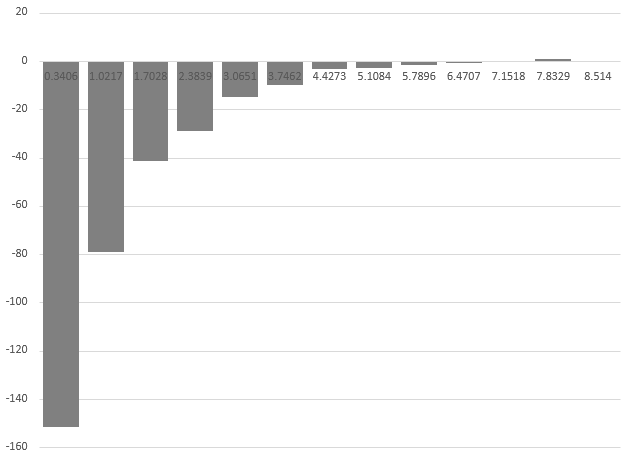
\includegraphics[height=8cm]{viseci-histogram-3.png}
    \caption{Viseči histogram.}
\end{figure}
%\begin{table}[H]
%    \centering
%    \begin{tabular}{c c}
%        \bf{Sredina intervala}  &	$\sqrt{n_j} - \sqrt{\hat{n_j}}$   \\
%        0.340561899  &	-0.289738214  \\
%        1.021685696  &	0.421112845 \\
%        1.702809493  &	0.683222035 \\
%        2.383933291  &	-0.552241845 \\
%        3.065057088  &	-0.098006028 \\
%        3.746180885  &	-1.312222049 \\
%        4.427304682  &	0.47329923 \\
%        5.10842848   &	-0.674672233 \\
%        5.789552277  &	-0.483766276 \\
%        6.470676074  &	-0.346879267 \\
%        7.151799872  &	-0.248725948 \\
%        7.832923669  &	0.821653805 \\
%        8.514047466  &	-0.12788117 \\
%    \end{tabular}
%    \caption{Tabela vrednosti $\sqrt{n_j} - \sqrt{\hat{n_j}}$.}
%\end{table}
\begin{table}[H]
    \centering
    \begin{tabular}{c c}
        \bf{Sredina intervala}  &	$\sqrt{n_j} - \sqrt{\hat{n_j}}$   \\
        0.3406   &	  -7.355883841   \\
        1.0217   &	  -5.00271844    \\
        1.7028   &	  -3.47106911    \\
        2.3839   &	  -3.727953988   \\
        3.0651   &	  -2.521344366   \\
        3.7462   &	  -3.158434944   \\
        4.4273   &	  -0.931138944   \\
        5.1084   &	  -1.741583517   \\
        5.7896   &	  -1.293244004   \\
        6.4707   &	  -0.960321451   \\
        7.1518   &	  -0.71310384    \\
        7.8329   &	  0.470472025    \\
        8.514    &	  -0.393210432   \\
    \end{tabular}
    \caption{Tabela vrednosti $\sqrt{n_j} - \sqrt{\hat{n_j}}$.}
\end{table}
\begin{figure}[H]
    \centering
    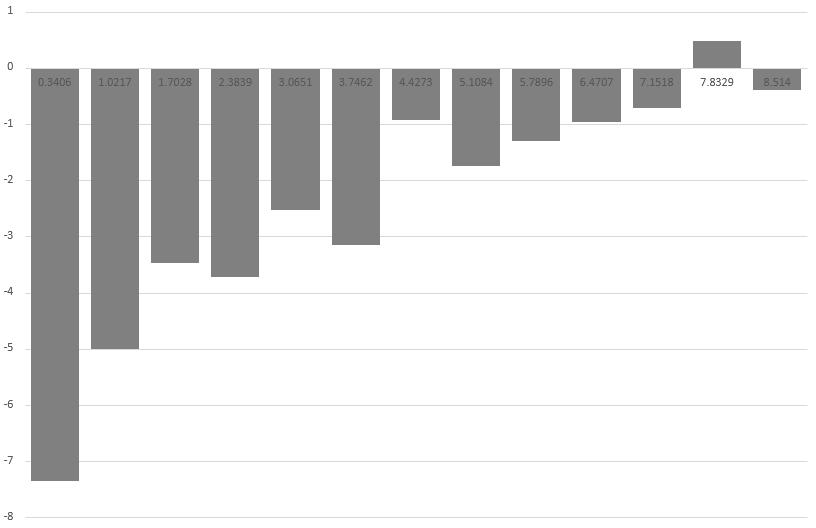
\includegraphics[height=8cm]{viseci-rootogram-3.png}
    \caption{Viseči histogram razlik korenov frekvenc.}
\end{figure}
Prednost visečega histograma razlik korenov frekvenc je, da se sosednji stolpci smejo v velikosti razlikovati
le malo, zato lahko hitro opazimo odstopanja. V našem primeru vidimo velika odstopanja na levi strani histograma.
%sredini histograma, ko razlika med dejansko frekvenco in pričakovano frekvenco pade pod $-1$. 
Pove nam, da 
smo opazili manj vrednosti kot smo jih pričakovali na danem intervalu. Še eno očitno odstopanje nastopi 
na desni, saj imamo dano eno trajanje $7{,}89$, kar je precej večje od povprečja.

Na koncu predstavimo rezultate še na logaritemski lestvici. Primerjalni kvantilni grafikon, v katerem primerjamo 
kvantile enakomerne porazdelitve s $F(X_k)$ je na logaritemski lestvici videti tako:
\begin{figure}[H]
    \centering
    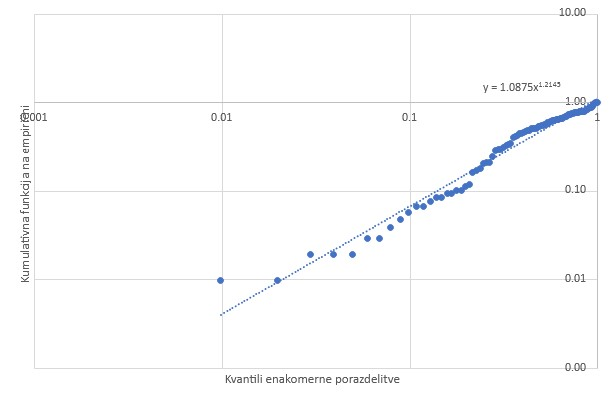
\includegraphics[height=8cm]{qq1log.jpg}
    \caption{Primerjalni kvantilni (Q--Q) grafikon na logaritemski lestvici.}
\end{figure}
Črta, ki se podatkom najbolje prilega je $y = 1{,}0875 x^{1{,}2145}$. V primeru, ko rišemo točke
$ \left( F^{-1} \left( \frac{k}{n+1}\right), X_k \right) $, pa je črta, ki se podatkom najbolje prilega 
na logaritemski lestvici $y = 0{,}9665 x^{1{,}1465}$, Q--Q grafikon pa je videti tako:
\begin{figure}[H]
    \centering
    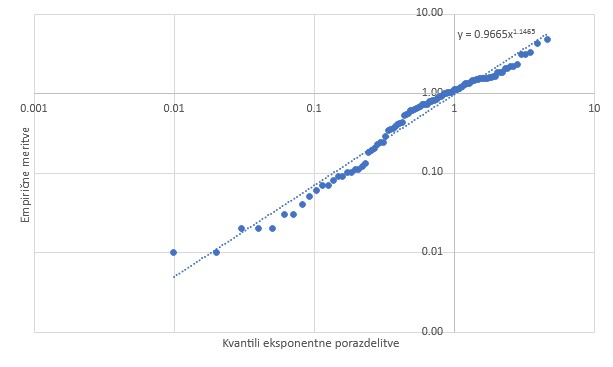
\includegraphics[height=8cm]{qq2log.jpg}
    \caption{Primerjalni kvantilni (Q--Q) grafikon v drugem primeru na logaritemski lestvici.}
\end{figure}

Ko s primerjalnim kvantilnim grafikonom primerjamo dve eksponentni porazdelitvi dobimo tudi na logaritemski
lestvici prileganje, ki zgleda linearno, v kolikor transformiramo tako abscizno kot tudi ordinatno os.


\section*{3. naloga: Temperature v Ljubljani}
V tej nalogi bomo konstruirali model linearne regresije in z njegovo pomočjo sklepali o segrevanju 
podnebja. Enostavna linearna regresija se ravna po predlogi $y = a + b x$, kjer je $x$ pojasnjevalna 
spremenljivka, $y$ odvisna spremenljivka, $a$ in $b$ pa iskana koeficienta. V našem primeru bomo najprej
z $X_i$ označevali leto, z $Y_i$ pa povprečno temperaturo tega leta. Te podatke združimo v tabelo.
\begin{table}[H]
    \centering
    \begin{tabular}{c c}
        \bf{Leto}  &	\bf{Povprečna temperatura}   \\
        1986  & 	9.533333333     \\
        1987  & 	9.616666667     \\
        1988  & 	10.525      \\
        1989  & 	10.45       \\
        1990  & 	10.675      \\
        1991  & 	9.95        \\
        1992  & 	11.13333333     \\
        1993  & 	10.59166667     \\
        1994  & 	11.825      \\
        1995  & 	10.75833333     \\
        1996  & 	9.775       \\
        1997  & 	10.775      \\
        1998  & 	11.01666667     \\
        1999  & 	10.975      \\
        2000  & 	12.175      \\
        2001  & 	11.39166667     \\
        2002  & 	11.80833333     \\
        2003  & 	11.575      \\
        2004  & 	10.66666667     \\
        2005  & 	10.425      \\
        2006  & 	11.4        \\
        2007  & 	12.05       \\
        2008  & 	11.56666667     \\
        2009  & 	11.68333333     \\
        2010  & 	10.68333333     \\
        2011  & 	11.75       \\
        2012  & 	12      \\
        2013  & 	11.6        \\
        2014  & 	12.64166667     \\
        2015  & 	12.15       \\
        2016  & 	11.75833333     \\
        2017  & 	11.91666667     \\
        2018  & 	12.48333333     \\
        2019  & 	12.54166667     \\
        2020  & 	12.11666667     \\
    \end{tabular}
    \caption{Tabela povprečnih temperatur v letih od $1986$ do $2020$.}
\end{table}
Model enostavne linearne regresije lahko zapišemo tudi z matrično enačbo $\bf{Y} = \bf{X} \beta + \epsilon$.
Tukaj je $Y$ slučajni, opažen vektor, $X$ deterministična matrika, $\beta$ determinističen, a neznan
vektor parametrov, $\epsilon$ pa slučajni in neznan vektor rezidualov. Matrična oblika modela enostavne 
linearna regresije je
\begin{gather}
    \label{matricni}
    \begin{bmatrix}
        Y_1 \\ ... \\ Yn
    \end{bmatrix}
    =
    \begin{bmatrix}
        1 & X_1 \\ ... & ... \\ 1 & X_n
    \end{bmatrix}
    \begin{bmatrix}
        a \\ b
    \end{bmatrix}
    +
    \begin{bmatrix}
        \epsilon_1 \\ ... \\ \epsilon_n
    \end{bmatrix} \text{.}
\end{gather}
Najboljša ocena za iskani $\beta$ v splošem je
$$ \hat{\beta} = \left( \bf{X}^T \bf{X} \right)^{-1} \bf{X}^T \bf{Y} \text{,} $$
ko upoštevamo \ref{matricni} pa se $\hat{\beta}$ posploši na
\begin{equation}
    \label{beta}
    \hat{\beta} = \frac{1}{n \sum X^2_i - \left( \sum X_i \right)^2 } 
    \begin{bmatrix}
        \sum X_i^2 \cdot \sum Y_i - \sum X_i \cdot \sum X_i Y_i  \\
        - \sum X_i \cdot \sum Y_i + n \sum X_i Y_i  \\
    \end{bmatrix} \text{,}
\end{equation}
kjer vsote tečejo po $i = 1 \dots n$.
Pri danih podatkih dobimo
\begin{equation*}
    \hat{\beta} = 
    \begin{bmatrix}
        \hat{a}\\ \hat{b}
    \end{bmatrix}
    = 
    \begin{bmatrix}
        - 118{,}2089496 \\
        0{,}064635854
    \end{bmatrix}\text{,}
\end{equation*}
kjer $\hat{b}$ predstavlja spremembo temperature v enem letu. Iz tega sledi, da bo temperatura narastla
za $1$ stopinjo v približno $15{,}5$ letih. Ocenimo standardno napako ocene naraščanja temperature $\hat{b}$.
Najprej izračunamo 
$$ \hat{\sigma}^2 = \frac{1}{n - 2} || Y - X \hat{b} ||^2 = \frac{1}{n - 2} \sum_{i=1}^{n} \hat{\epsilon}_i^2 \text{,}$$
kjer je $\hat{\epsilon}_i = Y_i - \hat{a} - \hat{b} X_i$. Dobimo $\hat{\sigma} = 0{,}52429844$. 
Če predpostavimo, da je šum porazdeljen večrazsežno normalno, sta cenilki $\hat{\beta}$ in $\hat{\sigma}^2$ 
neodvisni in velja  
$$ \frac{\bf{c}^T \hat{\beta} - \bf{c}^T \beta}{\hat{\sigma} \sqrt{\bf{c}^T \left( \bf{X}^T \bf{X} \right)^{-1} \bf{c}}} \approx \text{Student} \left( n - m\right)\text{,}$$
kjer je $\bf{c}$ determinističen vektor. Ko ocenjujemo $b$ upoštevamo, da je $\bf{c} = \left( 0, 1 \right)$ in dobimo
$$ \frac{\hat{b} - b}{\hat{\sigma}} \sqrt{\frac{n \sum X_i^2 - \left( \sum X_i\right)^2}{n}} \approx Student(n-2) \text{.}$$
Tako dobimo oceno standardne napake naraščanja temperature:
\begin{equation}
    \label{SE b}
    \Delta_b = \text{Student}_{1 - \frac{\alpha}{2}} \left( n - 2 \right) \frac{\hat{\sigma}}{\sqrt{\sum X_i^2 - \frac{1}{n} \left( \sum X_i \right)^2}} \approx 0{,}018126 \text{.}
\end{equation}
Ocena za strmino naraščanja temperature $\hat{b}$ je pozitivna, njena standardna napaka pa majhna, zato ni dvoma, da 
je linearni trend segrevanja statistično značilen.
V splošnem se standardna napaka izračuna kot
$$\text{SE} \left(\bf{c}^T \hat{\beta} \right) = \text{Student}_{1 + \frac{\alpha}{2}} \left( n - m \right) \hat{\sigma} \sqrt{\bf{c}^T \left( \bf{X}^T \bf{X} \right)^{-1} \bf{c}} \text{.}$$
Za standardno napako ocene koeficienta $a$ vstavimo $\bf{c} = \left( 1, 0 \right)$ in jo izračunamo kot
\begin{equation}
    \label{SE a}
    \Delta_a = \text{Student}_{1 - \frac{\alpha}{2}} \left( n-2 \right) \hat{\sigma} \sqrt{\frac{1}{n} + \frac{\left(\frac{1}{n} \sum X_{i}\right)^2}{\sum X_{i}^2 - \frac{1}{n} \left( \sum X_{i}\right)^2}} \approx 36{,}30595
\end{equation}
Napovejmo še povprečno temperaturo leta $2040$ in zanjo izračunajmo napovedni interval pri stopnji tveganja $\alpha = 0{,}05$.
Točkasta napoved za $Y$ je
\begin{equation}
    \label{napoved}
    \hat{Y} = \hat{a} + \hat{b} X = 13,6482 \text{,}
\end{equation}
kjer je $X = 2040$. Napovedni interval je potem enak $\hat{Y} - \Delta \leq Y \leq \hat{Y} + \Delta$,
kjer je 
\begin{equation}
    \label{Delta}
    \Delta = \text{Student}_{1 - \frac{\alpha}{2}} \left( n - 2 \right) \hat{\sigma} \sqrt{1 + \frac{1}{n} + \frac{\left( X - \frac{1}{n} \sum X_i \right)^2}{\sum X_i^2 - \frac{1}{n} \left( \sum X_i \right)^2}} \text{.}
\end{equation}
V našem primeru izračunamo $\Delta = 1{,}2869$, torej je interval zaupanja enak $ \left[ 12{,}3613, 14{,}9351 \right]$.

V drugem delu naloge bomo konstruirali model linearne regresija, pri čemer bomo vključili tudi letno nihanje temperature. 
V bistvu bomo konstruirali dvanajst modelov linearne regresije -- za vsak mesec enega -- podobno kot smo to storili zgoraj.
Naslednja tabela nam podaja povprečne mesečne temperature v letih od $1986$ do $2020$.
\begin{table}[H]
    \centering
    \begin{tabular}{c c c c c c c c c c c c c}
        \bf{Leto}  &	\bf{Jan}  &  \bf{Feb}  &  \bf{Mar}  &  \bf{Apr}  &  \bf{Maj}  &  \bf{Jun}  &  \bf{Jul}  &  \bf{Avg}  &  \bf{Sep}  &  \bf{Okt}  &  \bf{Nov}  &  \bf{Dec}  \\
        1986  &  0.1    &  -2.8  &  3.2   &  10.2  &  17.6  &  17.4  &  19.6  &  20.2  &  14.7  &  10.2  &  5.5  &  -1.5   \\                             
        1987  &  -3.4   &  0.5   &  1.1   &  11.1  &  13.3  &  17.8  &  21.4  &  18.7  &  18.3  &  11.2  &  4.5  &  0.9    \\                           
        1988  &  3.8    &  3.4   &  5.4   &  10.4  &  15.3  &  17.4  &  22    &  20.8  &  15.5  &  11.5  &  0.9  &  -0.1   \\                          	
        1989  &  -0.7   &  4.1   &  8.5   &  10.6  &  14.9  &  16.5  &  20.2  &  19.7  &  15.5  &  10.2  &  3.5  &  2.4    \\                           	
        1990  &  -0.5   &  5.7   &  8.8   &  9.1   &  16.2  &  17.7  &  20.2  &  20    &  14.1  &  11.3  &  5.1  &  0.4    \\                        	
        1991  &  0.7    &  -1.4  &  8.4   &  9.4   &  12.1  &  18.2  &  21.8  &  20.6  &  17.5  &  9.2   &  5.1  &  -2.2   \\                           
        1992  &  0.6    &  3.4   &  6.3   &  10.8  &  16.1  &  18.5  &  21.2  &  23.7  &  16.3  &  9.6   &  6.6  &  0.5    \\                          	
        1993  &  0.9    &  1     &  5.8   &  11.2  &  17    &  19.2  &  20.4  &  20.9  &  14.9  &  11.4  &  2.5  &  1.9    \\                       	
        1994  &  3.5    &  2.6   &  10.6  &  10.1  &  15.3  &  19.3  &  22.5  &  22.1  &  17.1  &  8.9   &  7.7  &  2.2    \\                           	
        1995  &  1   	&  4.5   &  5.1   &  11.3  &  15.1  &  17    &  22.8  &  19.1  &  14.3  &  12.3  &  5.3  &  1.3    \\                        
        1996  &  -0.8   &  -0.9  &  3.4   &  10.6  &  16    &  19.7  &  19.1  &  19.5  &  13.2  &  11    &  7.5  &  -1     \\                       
        1997  &  -0.5   &  4.1   &  7.5   &  8.5   &  16.3  &  19    &  20.1  &  20.2  &  16.6  &  9.6   &  5.3  &  2.6    \\                       	
        1998  &  3.2    &  5.3   &  5.8   &  11    &  15.8  &  20.7  &  21.5  &  21.6  &  15.6  &  11.4  &  3.4  &  -3.1   \\                          	
        1999  &  0.6    &  0.8   &  7.8   &  11.6  &  16.7  &  19.1  &  20.9  &  20.5  &  18.1  &  11.8  &  3.1  &  0.7    \\                           	
        2000  &  -1.6   &  4     &  7.6   &  13.6  &  17    &  20.9  &  19.9  &  22.1  &  16.4  &  12.9  &  8.4  &  4.9    \\                       	
        2001  &  3.4    &  4.7   &  8.8   &  10.1  &  17.2  &  18.4  &  21.9  &  22.9  &  13.8  &  14    &  3.6  &  -2.1   \\                          	
        2002  &  -0.6   &  5     &  8.9   &  10.1  &  17.3  &  21.1  &  21.3  &  20.1  &  15    &  11.5  &  9.4  &  2.6    \\                       	
        2003  &  -1.1   &  -0.9  &  7.4   &  10.3  &  18.3  &  23.5  &  22.6  &  24.2  &  15.5  &  8.8   &  8.2  &  2.1    \\                           	
        2004  &  -0.3   &  2.2   &  5     &  10.7  &  14    &  18.8  &  20.9  &  20.7  &  15.6  &  13    &  5.9  &  1.5    \\                     	
        2005  &  0.1    &  -0.3  &  5.7   &  10.8  &  16.3  &  19.5  &  21.1  &  18.4  &  16.4  &  11.8  &  5.1  &  0.2    \\                            	
        2006  &  -1.6   &  0.5   &  4.5   &  11.5  &  15.5  &  20.5  &  23.6  &  17.7  &  17.7  &  13.4  &  8.9  &  4.6    \\                           	
        2007  &  4.9    &  5.9   &  8.5   &  14.7  &  17.2  &  20.9  &  22    &  20.4  &  14.5  &  10.4  &  5.1  &  0.1    \\                         	
        2008  &  2.5    &  4.6   &  6.2   &  10.7  &  16.9  &  20.3  &  21.4  &  20.7  &  15.1  &  12    &  6.4  &  2      \\                       	
        2009  &  -1.5   &  2.3   &  7.1   &  13.3  &  18.1  &  18.9  &  21.7  &  22.4  &  17.4  &  11    &  7.5  &  2      \\                       	
        2010  &  -1.5   &  1.3   &  6.2   &  11.5  &  15.3  &  20.3  &  22.9  &  20.3  &  14.7  &  9.5   &  8.1  &  -0.4   \\                           	
        2011  &  1.5    &  1.5   &  7.1   &  13.5  &  17    &  20    &  21.1  &  22.8  &  19.4  &  10    &  3.8  &  3.3    \\                     	
        2012  &  1.6    &  -0.8  &  10.1  &  11.4  &  16.1  &  21.3  &  22.7  &  23.3  &  17    &  11.7  &  8.8  &  0.8    \\                          
        2013  &  2   	&  0.9   &  3.9   &  12.4  &  14.8  &  19.8  &  23.5  &  22.5  &  16.2  &  13.2  &  7.3  &  2.7    \\                          
        2014  &  5.4    &  4.4   &  10    &  13.1  &  15.7  &  20.2  &  20.8  &  19.6  &  16.2  &  13.6  &  8.8  &  3.9    \\                          	
        2015  &  2.8    &  2.4   &  7.6   &  11.8  &  17    &  20.6  &  24.3  &  22.3  &  16.5  &  11    &  6.9  &  2.6    \\                       	
        2016  &  1.1    &  5.5   &  7.5   &  12.5  &  15.3  &  20    &  23.2  &  20.6  &  18.3  &  10.3  &  7    &  -0.2   \\                        	
        2017  &  -3.2   &  4.5   &  10.2  &  12.1  &  16.9  &  21.7  &  23.2  &  23.2  &  14.3  &  12    &  6.2  &  1.9    \\                          	
        2018  &  4.8    &  -0.1  &  4.6   &  15.2  &  18    &  20.9  &  22.3  &  22.8  &  17.6  &  13.2  &  8.3  &  2.2    \\                          	
        2019  &  0.7    &  4.9   &  9     &  11.6  &  12.9  &  23.5  &  22.9  &  22.6  &  16.8  &  13.2  &  8.8  &  3.6    \\                         	
        2020  &  1.9    &  6.8   &  7.2   &  13    &  15.3  &  19.6  &  21.8  &  22.2  &  17.5  &  11.9  &  5.3  &  2.9    \\                         	
    \end{tabular}
    \caption{Tabela povprečnih mesečnih temperatur v letih od $1986$ do $2020$.}
\end{table}

Tako kot prej bomo s formulo \ref{beta} ocenili koeficiente za vsakega od modelov. Označimo z $\beta_j$ koeficiente modela
$j$-tega meseca. Če sedaj $X_{ij}$ označuje $j$-ti mesec $i$-tega leta, $Y_{ij}$ pa pripadajočo temperaturo, oceno za koeficiente
izračunamo z 
\begin{equation*}
    \hat{\beta_j} = \frac{1}{n \sum X^2_{ij} - \left( \sum X_{ij} \right)^2 } 
    \begin{bmatrix}
        \sum X_{ij}^2 \cdot \sum Y_{ij} - \sum X_{ij} \cdot \sum X_{ij} Y_{ij}  \\
        - \sum X_i{ij} \cdot \sum Y_{ij} + n \sum X_{ij} Y_{ij}  \\
    \end{bmatrix} \text{,}
\end{equation*}
kjer vse vsote spet tečejo po letih $i = 1 \dots n\text{, } n = 35$. V naslednji tabeli so 
zbrane ocene koeficientov 
$\hat{\beta_i} = 
\begin{bmatrix}
    \hat{a_i}\\
    \hat{b_i}
\end{bmatrix}$,
ter standardne napake teh ocen po formulah \ref{SE b} in \ref{SE a}.

\begin{table}[H]
    \centering
    \begin{tabular}{c c c c c c c c c c c c c}
        &	\bf{Jan}  &  \bf{Feb}  &  \bf{Mar}  &  \bf{Apr}   \\
        $\hat{a_i}$       &  -94.19288515  &	-100.2831092  &	-114.0293838  &	-173.6722969   \\
        $\hat{b_i}$       &  0.04745098	&  0.051344538  &	0.060364146  &	0.092408964   \\
        $SE (\hat{a_i})$  &  855.482328  &	963.9493216  &	839.0534516  & 	461.6688106    \\
        $SE (\hat{b_i})$  &  0.427095084  &	0.481246664  & 	0.418893053  &	0.230485742    \\
        &  \bf{Maj}  & \bf{Jun}  &  \bf{Jul}  &  \bf{Avg}   \\
        $\hat{a_i}$       &  -23.22411765  & 	-197.3568627  &  	-113.4804202 &	-95.12683473  \\
        $\hat{b_i}$       &	0.019579832  & 	0.108347339  &	0.067478992  &	0.058039216    \\ 
        $SE (\hat{a_i})$  &	563.4320175  &	468.8558869  &	406.9318144  &	590.9713987   \\
        $SE (\hat{b_i})$  &	0.281290492  &	0.234073853  &	0.203158583  &	0.295039384  \\
        &  \bf{Sep}  &  \bf{Okt}  &  \bf{Nov}  &  \bf{Dec}  \\
        $\hat{a_i}$       &  -62.89501401 &	-91.2472549  &  -202.607395  &	-150.3918207  \\
        $\hat{b_i}$       &	0.039439776  &	0.051232493  &  0.104201681  &	0.075742297  \\
        $SE (\hat{a_i})$  &	563.7060539  &	521.614813   &  727.0058193  &	690.5996253  \\
        $SE (\hat{b_i})$  &	0.281427303  &	0.260413471  &  0.362953858  &	0.344778256  \\
    \end{tabular}
    \caption{Ocene koeficientov in njihove standardne napake}
\end{table}
Hitro vidimo, da so napake koeficientov v tem primeru precej večje kot v prejšnjem modelu. 
To nam pove, da temperature v, na primer, januarju skozi leta nihajo in je zanje težko predpisati 
linearno črto, h kateri strmijo, kot smo to naredili za povprečne letne temperature. Kljub temu dajmo 
napovedati pričakovano januarsko temperaturo za leto $2040$, kot to od nas zahteva naloga.  
Z uporabo formul \ref{napoved} in \ref{Delta} izračunamo, da leta $2040$ v januarju pričakujemo
$2{,}6071$ stopinj, z verjetnostjo $0{,}95$ pa bo povprečna temperatura padla med $2{,}0856$ in 
$3{,}1287$ stopinj.



\end{document}